\chapter{2D case}
\label{chapter:2d}

% {{{1 INTRODUCTION
\section{Introduction}

In this part, we focus on point clouds in 2D which sample a planar curve.  We
will develop algorithms to smooth them by minimizing different energies. First,
we will consider for the energy the area of a union of disks centered on the
point cloud.  We will also test other types of energies such as the perimeter of
the boundary, a weighted area and a weighted perimeter of the boundary.

Firstly, we will explain how to compute the area of a union of disks.  Then, we
will run different experiments to check that the gradient of a union of disks is
proportional to the mean curvature of the underlying curve. Finally, we will run
our flows on different point clouds with different parameters to show that it
can simulate discrete mean curvature flows and indeed smooth point clouds.

% {{{1 AREA OF A UNION OF BALLS
\section{Area of a union of balls}

Let $ P $ be a finite set of points in 2D.  We call the union of disks with
radius $ r $ centered on $ P $, the $r$-offset and we will denote it by $ P^r $.
We will first need the definition of the Voronoi diagram of set of points:

\begin{definition}
    Given a set of points $ P \subseteq \R^2 $ also called sites, we define the
    Voronoi cell of $ p \in P $ by:
    $$ V(p, P) = \{ x \in \R^2,~ \forall p' \in P,~|| p  - x || \leq || p' -
    x || \} $$
    In other words, the Voronoi cell of $ p $ is composed of all the points
    which are closer to $ p $ than to any other points in $ P $.  Then, the
    Voronoi diagram of $ P $ is composed of all the Voronoi cells of $ p \in P
    $. It defines a partition of the plane $ \R^2 $.
\end{definition}

For example, Figure \ref{fig:voronoi-diagram-2d} provides an example of Voronoi
diagram. Now, we can say that, because the Voronoi diagram defines a partition,
we have:

\begin{equation}
    Area(P^r) = Area \left( \bigcup_p B(p, r) \right) = \sum_p Area(V(p, P) \cap B(p, r))
    \label{eqn:area-union-balls}
\end{equation}

\begin{figure}[h]
    \centering
    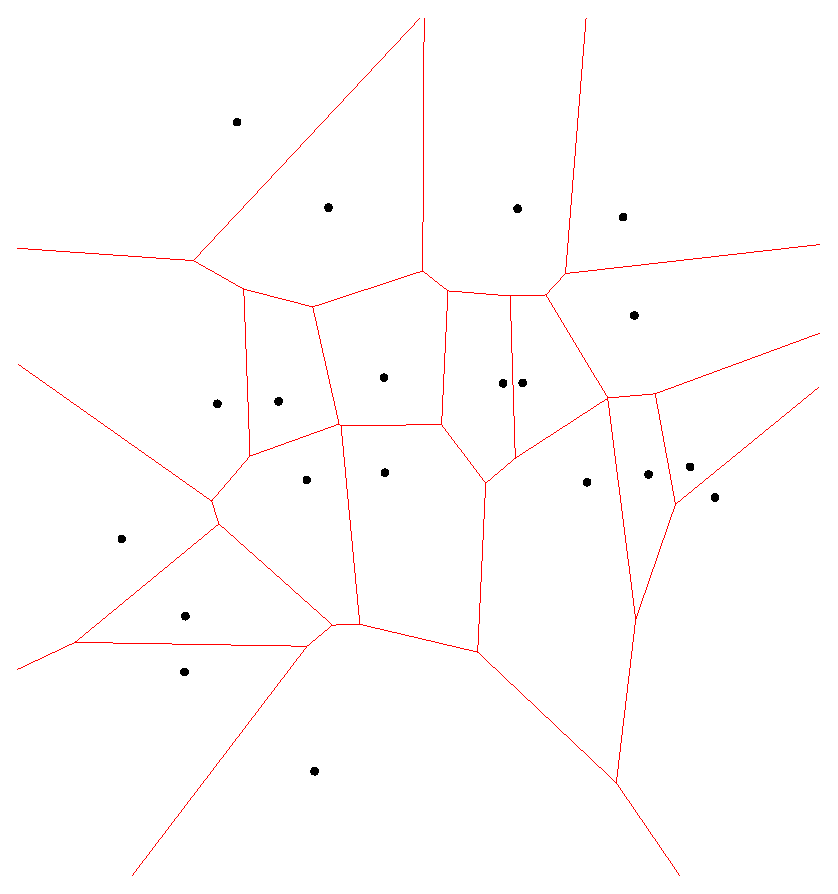
\includegraphics[scale=0.4]{voronoi-diagram-2d}
    \caption{Points are in black and the boundary of the Voronoi cells are in
        red}
    \label{fig:voronoi-diagram-2d}
\end{figure}

% {{{3 ALGORITHM
\paragraph{Algorithm}

In order to compute this quantity, we need to know how to estimate the area of
the intersection of a ball and a Voronoi cell. Figure
\ref{fig:inter_voronoi_ball_2d} illustrates different cases we may encounter
when intersecting a Voronoi cell and a ball in 2D.

\begin{figure}[h]
    \centering
    \begin{minipage}{0.32\linewidth}
        \centering
        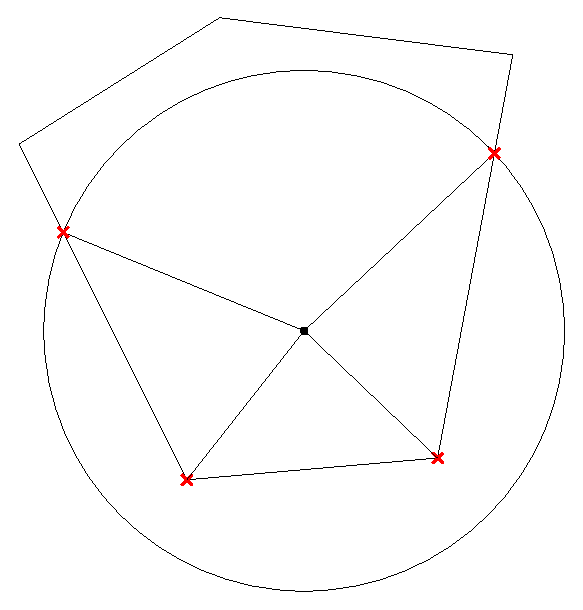
\includegraphics[scale=0.4]{2d/inter_voronoi_ball_2d}
        \subcaption{General case}
        \label{fig:inter_voronoi_ball_2d:a}
    \end{minipage}
    \begin{minipage}{0.32\linewidth}
        \centering
        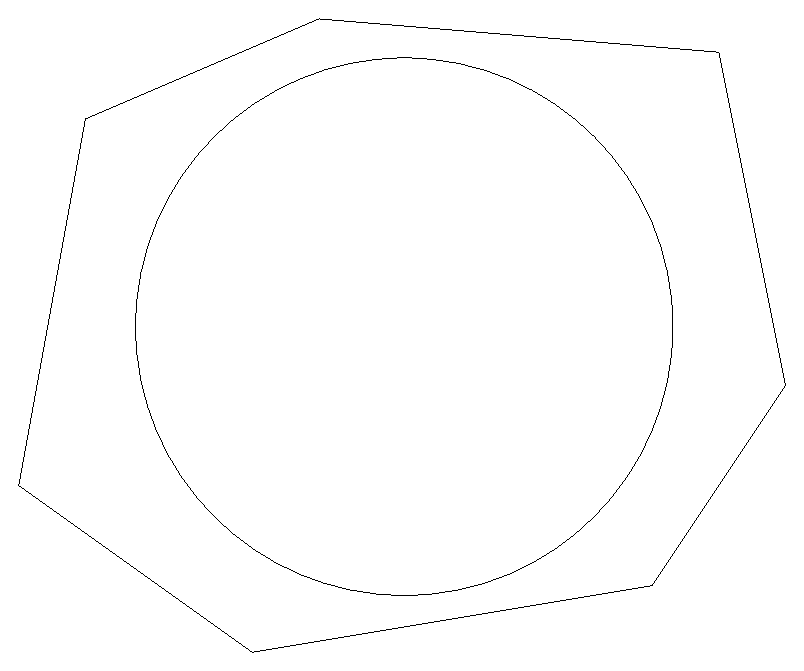
\includegraphics[scale=0.4]{2d/inter_voronoi_ball_2d_no_inter}
        \subcaption{No intersections}
        \label{fig:inter_voronoi_ball_2d:b}
    \end{minipage}
    \begin{minipage}{0.32\linewidth}
        \centering
        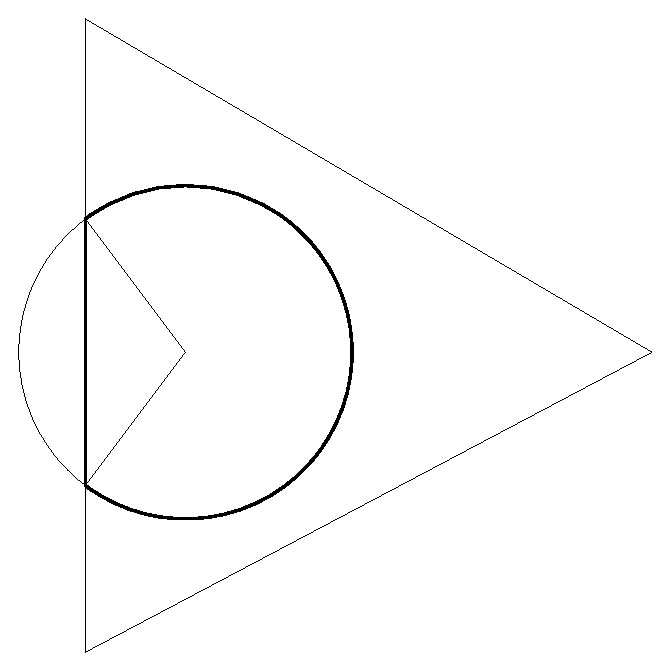
\includegraphics[scale=0.4]{2d/inter_voronoi_ball_2d_2_inter}
        \subcaption{2 intersections}
        \label{fig:inter_voronoi_ball_2d:c}
    \end{minipage}

   \caption{Different cases for the intersection between a Voronoi cell and a
       disk}
   \label{fig:inter_voronoi_ball_2d}
\end{figure}

We use \texttt{CGAL} to compute the Delaunay triangulation of our point set: it
is the dual of the Voronoi diagram. A triangle in the Delaunay
triangulation corresponds to a vertex in the Voronoi diagram, an edge
corresponds to an edge, a site corresponds to a face...

Given this triangulation, we can compute the vertices composing the boundary of
the  Voronoi cell of a point by doing the following:
\begin{enumerate}
    \item Access the neighbouring faces of a site using the
        \texttt{incident\_faces} method.
    \item Compute the Voronoi vertices (circumcenters) of these faces using the
        \texttt{dual} method.
\end{enumerate}

We are now ready to compute the intersection of the Voronoi cell of $ p $ and a
ball $ B(p, r) $. The boundary of this intersection is composed of segments and
circular arcs. There are two types of points connecting those elements: some are
Voronoi vertices (in red) and some are intersections of Voronoi edges and
circular arcs (in blue). We will refer to the red points as the interior points
and to the blue ones as intersection points.

First, we construct an array of all the points composing the boundary of the
intersection. In order to do this, we loop over the vertices composing the
Voronoi cell: for any Voronoi vertex $ v $, we have access to the next one in
the counterclockwise order and so we construct the corresponding edge. We check
whether this edge intersects the ball or not and we construct the intersection
points if necessary. In parallel, we maintain a boolean indicating whether the
current vertex is interior or not to $ B(p, r) $. By doing that, we can
construct an ordered list of all blue and red the points present on the boundary
of the intersection.

Then, we loop over this array. For any two consecutive points $ u $ and $ v $,
we can construct the edge $ e = uv $. Depending on whether the points $ u $ and
$ v $ are interior or not, the contribution of $ e $ to the global area will be
different:
\begin{itemize}
    \item if $ u $ and $ v $ are interior points, we add the area of triangle $ upv $.
    \item if $ u $ or $ v $ is interior point, we add the area of triangle $ upv $.
    \item if $ u $ and $ v $ are intersection points, then if they belong to the
        same Voronoi edge, we add the area of triangle $ upv $. If not, we add the
        area of angular sector $ \vec{pu}, \vec{pv} $.
\end{itemize}

Some special cases need to be handled:
\begin{itemize}
    \item the boundary of the Voronoi cell lies entirely outside the ball, then
        we add $ \pi r^2 $ to the area of the union (see Figure
        \ref{fig:inter_voronoi_ball_2d:b}).
    \item the boundary consists of two intersection points $ p $ and $ q $, then
        we add the triangle $ pvq $ and the angular sector $ \vec{vp}, \vec{vq}
        $ (see Figure \ref{fig:inter_voronoi_ball_2d:c}).
    \item there is only one point on the boundary (can happen if adjacent balls
        are tangential), then we add $ \pi r^2 $.
\end{itemize}

This algorithm allows us to compute exactly the area of a union of disks.

We use the same technique for computing the contribution of each disk $ B(p, r)
$ to the perimeter of the boundary of the union of disks except that if $ B(p,
r) $ is contained in $ V(p, P) $ then the contribution to the perimeter is $ 2
\pi r $ and instead of adding triangles areas or angular sectors, we only add
length of circular arcs.

% {{{3 IMPLEMENTATION DETAILS
\paragraph{Implementation details}

For the implementation, we used different libraries: \texttt{CGAL} which is a
C++ library that offers all the basic geometric types (point, vector, line,
plane..), data structures and algorithms (triangulations...). We also used
\texttt{Eigen} which is a C++ linear algebra library which provides types such
as vector, matrix and manipulation operations. We used \texttt{Qt} for the GUI
programming.

The main difficulty here was to compute the intersection between a Voronoi cell
and a circle. The Voronoi cell is computed using its dual graph: the Delaunay
triangulation. The intersection procedure was described previously.

We also used the automatic differentiation technique (see Appendix
\appendixref{appendix:ad}): it allowed us to only worry about the computation of the
area and not of its gradient.

% {{{1 EXPERIMENTS
\section{Experiments}

% {{{2 GRADIENT
\subsection{Gradient}

In this section, we will illustrate on some examples what gives the computation
of the gradient of the area of union of balls and the gradient of the perimeter
of the boundary. We used the automatic differentiation technique described in
Appendix \appendixref{appendix:ad}.

See Figure \ref{fig:gradients_area_2d} for a few examples of such gradients
for different input point sets. The colour of the vector depend on the norm of
the gradient: the bigger the gradient is, the redder the vector will be.

\begin{figure}[h]
    \centering

    \includegraphics[scale=0.3]{2d/area/ellipse-100-01-15-gradients}
    \includegraphics[scale=0.3]{2d/area/square-40-001-100-gradients}
    \caption{Gradients of the area for points on an ellipse (left) and on a
        square (right)}
    \label{fig:gradients_area_2d}
\end{figure}

We did the same thing with the gradient of the perimeter of the boundary on the
same point clouds (see Figures \ref{fig:gradients_perimeter_2d}).

\begin{figure}[h]
    \centering
    \includegraphics[scale=0.3]{2d/perimeter/ellipse-100-01-15-gradients}
    \includegraphics[scale=0.3]{2d/perimeter/square-40-001-100-gradients}

    \caption{Gradients of the perimeter for points on an ellipse (left) and on a
        square (right)}
    \label{fig:gradients_perimeter_2d}
\end{figure}

In the previous screenshots, we observe that the gradients are in the same
direction as the normals to the underlying curve. This is the case if the radii
of the balls are big enough and if the sampling is sufficiently uniform. Also,
the norm of these gradients is related to the mean curvature of the underlying
curve (see Proposition \ref{prop:gradient-mean-curvature}).

% {{{2 MEAN CURVATURE ESTIMATION
\subsection{Mean curvature estimation}

In this section, we experimentally check in a particular case that we can
estimate the mean curvature on a point set using the norm of the gradients of
the area of a union of disks. The theoretical justification is given in chapter
\ref{chapter:theory}.

We run our tests on a sampled ellipse whose major and minor axes are $ a $ and $
b $. We can parametrize this ellipse by :
$$
\begin{cases}
    x(t) &= a \cos (t) \\
    y(t) &= b \sin (t)
\end{cases}
\text{ for t } \in [ 0, 2\pi ]
$$

We recall the formula for computing the curvature of a parametrized curve:
\begin{equation}
    \kappa(t) = \frac{x'(t) y''(t) - y'(t) x''(t)}{(x'^2(t) +
        y'^2(t))^{\frac{3}{2}} }
\end{equation}

For an ellipse, we obtain:
$$ \kappa(t) = \frac{ab}{(a^2 \cos^2(t) + b^2 \sin^2(t))^{\frac{3}{2}} } $$

We compare this for $ t = \frac{2 k \pi}{N} $ for $ k = 0 \ldots N - 1 $ with
the computed ones where $ N $ is the number of samples.

Figure \ref{fig:2d-curvature-ellipse} represents the computed gradients mapped
to a colour ramp (from green to red). We observe that the gradients are more
important where the curvature is higher and are collinear to the outward normals
of the underlying curve.

\begin{figure}[h]
    \centering

    \includegraphics[scale=0.3]{2d/area/curvature-ellipse-200-15}
    \includegraphics[scale=0.3]{2d/perimeter/curvature-ellipse-200-15}
    \caption{Computed curvatures on an ellipse using gradients of the area /
        perimeter}
    \label{fig:2d-curvature-ellipse}
\end{figure}

Now, we study the absolute difference between the computed and expected
curvatures for different choices of gradients (area, perimeter of the boundary,
weighted...), see Figure \ref{fig:2d-curvature-error-ellipse}.

\begin{figure}[h]
    \centering

    \includegraphics[scale=0.3]{2d/area/curvature-error-ellipse-200-05}
    \includegraphics[scale=0.3]{2d/perimeter/curvature-error-ellipse-200-05}
    \caption{Error between the curvatures on an ellipse using gradients of the
        area / perimeter}
    \label{fig:2d-curvature-error-ellipse}
\end{figure}

We see that the error is less important for the area.

% {{{2 DISCRETE MEAN CURVATURE FLOW
\subsection{Discrete Mean Curvature Flow}

Now, we will be interested in approximating the continuous mean curvature flow
by applying a gradient descent algorithm in order to minimize a functional $ E
$. This gradient descent will be done using a constant timestep (Euler explicit
scheme).

We will also be interested in weighted versions of functionals: we can weight
the gradient of the area by the perimeter of the visible part (the circular arcs
composing the intersection of the Voronoi cell and the ball) of the restricted
region. But by doing that, we can divide by $ 0 $ so we need to choose a small
time step in order to avoid the case where the contribution of a site to the
perimeter vanishes.

We will test the different properties we expect the flows to have:
\begin{enumerate}
    \item Smooth the point clouds: remove outliers, noise
    \item Minimize the area of a union of balls
\end{enumerate}

We did some experiments to validate our results: we first compared the two
gradient flows (area and perimeter of the boundary) to a set of points uniformly
sampled on an ellipse, see Figure \ref{fig:ellipse_flows}.

% TODO: ajouter convergence vers cercle
\begin{figure}[h]
    \centering

    \includegraphics[scale=0.3]{2d/ellipse-balls-15}
    \includegraphics[scale=0.3]{2d/area/ellipse-100-01-15-100}
    \includegraphics[scale=0.3]{2d/perimeter/ellipse-100-01-15-100}
    \caption{Area / perimeter flow of an ellipse: 100 iterations}
    \label{fig:ellipse_flows}
\end{figure}

\paragraph{Smoothing}

We also run the perimeter flow on point clouds such as a bird (Figure
\ref{fig:bird_perimeter_flow}), a shark (Figure \ref{fig:shark_perimeter_flow})
and a square (Figure \ref{fig:area_perimeter_flow_square}) to observe the
smoothing effect of the flows.

\begin{figure}[h]
    \centering

    \begin{subfigure}[b]{\textwidth}
        \includegraphics[scale=0.25]{2d/perimeter/shark-0}
        \includegraphics[scale=0.25]{2d/perimeter/shark-24}
        \includegraphics[scale=0.25]{2d/perimeter/shark-49}
        \subcaption{Shark: 0 / 25 / 50 iterations}
        \label{fig:shark_perimeter_flow}
    \end{subfigure}

    \begin{subfigure}[b]{\textwidth}
        \includegraphics[scale=0.25]{2d/perimeter/bird-0}
        \includegraphics[scale=0.25]{2d/perimeter/bird-24}
        \includegraphics[scale=0.25]{2d/perimeter/bird-49}
        \caption{Bird: 0 / 25 / 50 iterations}
        \label{fig:bird_perimeter_flow}
    \end{subfigure}

    \caption{Examples of perimeter flows}
\end{figure}

\begin{figure}[h]
    \centering
    \includegraphics[scale=0.3]{2d/square-0}
    \includegraphics[scale=0.3]{2d/area/square-area-4-15-01}
    \includegraphics[scale=0.3]{2d/perimeter/square-perimeter-10-15-05}
    \caption{Area / perimeter flow on a square}
    \label{fig:area_perimeter_flow_square}
\end{figure}

Next, we add some outliers around the ellipse and observe the effects of the two
flows: see Figure \ref{fig:ellipse_outliers_flow}. We see that the outliers
are "swallowed" by the initial point set in both cases. But, for the area flow,
a hole is created at the same place where the outliers were added.

\begin{figure}[h]
    \centering

    \includegraphics[scale=0.3]{2d/area/ellipse-100-01-15-outliers}
    \includegraphics[scale=0.3]{2d/area/ellipse-100-01-15-outliers-40}
    \includegraphics[scale=0.3]{2d/perimeter/ellipse-100-1-15-outliers-100}
    \caption{Area / perimeter flow of an ellipse with outliers}
    \label{fig:ellipse_outliers_flow}
\end{figure}

Furthermore, we added Gaussian noise on these points to test the robustness
of our algorithm, see Figure \ref{fig:ellipse_noise_flow}.

\begin{figure}[h]
    \centering

    \includegraphics[scale=0.3]{2d/ellipse-noise-5-0}
    \includegraphics[scale=0.3]{2d/area/ellipse-noise-5-75}
    \includegraphics[scale=0.3]{2d/perimeter/ellipse-noise-5-75}
    \caption{Area /perimeter flow on a noised ellipse}

    \label{fig:ellipse_noise_flow}
\end{figure}

We notice that the gradient flow of the area may create holes in the point set
which is not the case for the gradient flow of the perimeter.  On the contrary,
the gradient flow of the perimeter of the boundary will smooth the point set
while redistributing the points in an uniform way.  This can be explained by
looking to a simple case with two intersecting balls:
\begin{itemize}
    \item \textit{for the perimeter}: the gradients are directed towards the
        outside and so the balls will be merged because it is easy to see, using
        the triangle inequality, that in order to minimize the perimeter the
        balls must come closer.
    \item \textit{for the area}: it is possible that, in order to minimize the
        area, we gain more by moving the balls apart rather than closer.
\end{itemize}

The chosen radius will also influence the smoothing: points which are too far
away from other points (at distance greater than the radius) will not move. The
bigger the radius is, the more points will move in big groups. Indeed, the
radius indicates how to take the neighbours of a point into account. The more
neighbours we take into account, the more "global" the movement will be.

We also add varying oscillations to our ellipse in order to see the adaptive
part of the algorithm. We generate oscillations with one or two amplitudes. For
one constant amplitude, see Figure \ref{fig:ellipse_osc_flow}. For two
different amplitudes see Figure \ref{fig:ellipse_osc2_flow}.

\begin{figure}[h]
    \centering

    \includegraphics[scale=0.3]{2d/ellipse-osc-25-15-0}
    \includegraphics[scale=0.3]{2d/area/ellipse-osc-25-15-25}
    \includegraphics[scale=0.3]{2d/perimeter/ellipse-osc-25-15-50}
    \caption{Area / perimeter flow on an ellipse with oscillations (one
        amplitude)}

    \label{fig:ellipse_osc_flow}
\end{figure}

\begin{figure}[h]
    \centering

    \includegraphics[scale=0.3]{2d/ellipse-osc2-20}
    \includegraphics[scale=0.3]{2d/area/ellipse-osc2-20-15-25}
    \includegraphics[scale=0.3]{2d/perimeter/ellipse-osc2-20-15-55}
    \caption{Area /perimeter flow on an ellipse with oscillations (two
        amplitudes)}

    \label{fig:ellipse_osc2_flow}
\end{figure}

Lastly, we generate points on a line segment and fixed the two points of the
extremities. Then, we apply our flow on this point set. We expect the flow to
smooth the point set: points should get closer and closer to an uniformly
sampled set of points. See Figure \ref{fig:line_fixed_flow}.

\begin{figure}[h]
    \centering

    \includegraphics[scale=0.5]{2d/area/line-01-15-0}
    \includegraphics[scale=0.5]{2d/area/line-01-15-50}
    \includegraphics[scale=0.5]{2d/perimeter/line-05-15-50}
    \caption{Left: Initial point set. Middle and right: area / perimeter flow of
        points on a segment after 50 iterations}

    \label{fig:line_fixed_flow}
\end{figure}

\paragraph{Minimization}

We also check that the area of a union of balls decreases with the number of
iterations, see Figure \ref{fig:area_time_decrease}.

\begin{figure}[h]
    \centering
    \includegraphics[scale=0.3]{2d/values-square-area}
    \includegraphics[scale=0.3]{2d/values-ellipse-perimeter}
    \caption{Evolution of the area on different point clouds with the area
        flow : square / ellipse}
    \label{fig:area_time_decrease}
\end{figure}

% {{{1 CONCLUSION
\section{Conclusion}

In summary, the two flows (area and perimeter of the boundary) have the
following common properties:
\begin{itemize}
    \item Smooth the point set: remove the outliers / noise
    \item Can be used to estimate the mean curvature
\end{itemize}

But, there are differences between the two flows. The main one is that the area
flow has the tendency to create holes in the point cloud. This difference is
removed when we use the weighted versions of the flows.

% {{{1 ASSESSMENT
% \section{Assessment}

% In this chapter, we saw how to simulate discrete mean curvature flows by using
% the gradient of the volume of the $r$-offset of a point cloud.

% Also, we want to use polyhedral (anisotropic) norms, a thing that the previous
% method does not allow since it only deals with intersection of a Voronoi cell
% and a ball and we need a way to intersect a Voronoi cell and a polygon.

% vim: set spelllang=en :
